\title{A Constrained Optimization Problem}
\subtitle{\SubTitleName}
\institute[]{\Course}
\author{\Instructor}
\maketitle   
   

\frame{\frametitle{Topics and Objectives}
\Emph{Topics} \\
%\TopicStatement
\begin{itemize}

    \item constrained optimization as an eigenvalue problem
    % \item distance and orthogonality constraints

\end{itemize}

\vspace{0.5cm}

\Emph{Learning Objectives}\\

%\LearningObjectiveStatement

\begin{itemize}

    \item apply eigenvalues and eigenvectors to solve a class of optimization problems that are subject to a distance constraint % and orthogonality constraints.
    
\end{itemize}

} 


\begin{frame}\frametitle{Temperature on a Sphere}

    \begin{minipage}{.58\textwidth}
        The surface of a unit sphere in $\mathbb R^3$ is given by $$ 1 = x_1^2 + x_2^2 + x_3^2 = ||\vec x||^2$$ 
        \pause $Q$ is a quantity (for example, temperature) that we want to optimize $$Q(\vec x) = 9x_1^2 + 4x_2^2 +3x_3^2$$ 
    \end{minipage} \begin{minipage}{.41\textwidth}
    \begin{center}
        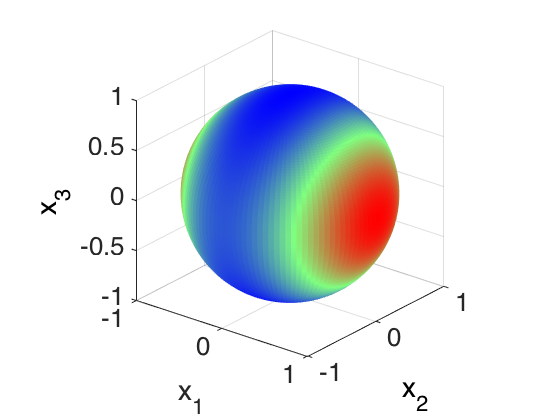
\includegraphics[width=1\textwidth]{Chapter7/images/sphere73.png} 
    \end{center}
    \end{minipage} 
    
    \vspace{12pt} 
    \pause 
    Identify the largest and smallest values of $Q$ on the surface of the sphere, and where they are located. 
    
\end{frame}


\begin{frame}\frametitle{Solution: Largest Value of $Q$ on Sphere}    
    We will identify the largest value of $Q$ on the sphere first. 
    \begin{align*}
        Q =  \vec x\, ^T \spalignmat{9 0 0;0 4 0;0 0 3}\vec x &= 9x_1^2 + 4x_2^2 +3x_3^2 \\
        &\le 9x_1^2 + 9x_2^2 +9x_3^2 \\
        &= \onslide<2->{ 9 (x_1^2 + x_2^2 +x_3^2)} \\
        &= \onslide<3->{9 \lVert \vec x \rVert ^2} \\
        &= \onslide<4->{ 9  }
    \end{align*}
    \onslide<5->{We are only considering points on the surface of the sphere: $\lVert \vec x \rVert ^2 = 1$.  }
\end{frame}


\begin{frame}\frametitle{Solution: Largest and Smallest Values of $Q$ on Sphere}     
    \onslide<2-> {Thus, $$\mathrm{max} \{ Q(\vec x) : ||\vec x|| = 1\} = 9, \ \text{and max occurs at } \vec x = \spalignmat{\pm1;0;0}$$}
    \onslide<3-> {A similar analysis yields 
    $$\mathrm{min} \{ Q(\vec x) : ||\vec x|| = 1\} = 3, \ \text{and min occurs at } \vec x = \spalignmat{0;0;\pm1}$$}
    \onslide<4->{Notice that the minimum and maximum values of $Q$ were the eigenvalues of $A$, and the corresponding eigenvectors gave their locations.}
\end{frame}


\begin{frame}\frametitle{A Constrained Optimization Problem}

    Suppose we wish to find the maximum or minimum values of $$Q(\vec x) = \vec x^{\, T}A \vec x, \quad \vec x \in \mathbb R^n, \quad A \in \mathbb R^{n\times n},$$ subject to $$||\vec x|| = 1$$ \pause That is, we want to find
    \begin{align*}
        m &= \mathrm{min} \{ Q(\vec x) : ||\vec x|| = 1 \} \\
        M &= \mathrm{max} \{ Q(\vec x) : ||\vec x|| = 1 \}
    \end{align*}
    \pause 
    This is an example of a \Emph{constrained optimization} problem. Note that we may also want to know where these extreme values are obtained. 
    
\end{frame}


\begin{frame}\frametitle{Constrained Optimization and Eigenvalues}
    
    \begin{center}\begin{tikzpicture} \node [mybox](box){\begin{minipage}{0.95\textwidth}\vspace{2pt}
    
        If $Q = \vec x^{\, T} A \vec x$, $A$ is a real $n\times n$ symmetric matrix, with eigenvalues 
        $$\lambda_1 \ge \lambda_2 \ldots \ge \lambda_n$$
        and associated normalized eigenvectors 
        $$\vec u_1, \vec u_2, \ldots , \vec u_n$$
        \onslide<2->{Then, subject to the constraint $||\vec x ||=1$, }
        \begin{itemize}
            \item<3-> the \Emph{maximum} value of $Q(\vec x) = \lambda_1$, attained at $\vec x = \pm \, \vec u_1$.
            \item<4-> the \Emph{minimum} value of $Q(\vec x) = \lambda_n$, attained at $\vec x = \pm \, \vec u_n$.
        \end{itemize} 
        
    \end{minipage}};
    \node[fancytitle, right=10pt] at (box.north west) {Theorem};
    \end{tikzpicture}\end{center}
    

\end{frame}


\begin{frame}\frametitle{Proof for Maximum Value of $Q$}
    
    Assume $\lambda_1$ is the largest eigenvalue with corresponding unit eigenvector $\vec u_1$. 
    \begin{align*}
        \onslide<2->{Q = \vec x \,^T A\vec x 
                 &= \vec y\, ^T D\vec y , \quad \text{using } A = PDP^T , \ \vec x = P\vec y\\}
        \onslide<3->{&= \sum \lambda_i y_i^2, \quad \text{because } D \text{ is diagonal} \\}
        \onslide<4->{&\le \sum \lambda_1 y_i^2, \quad \text{because } \lambda_1 \text{ is the largest eigenvalue} \\}
        \onslide<5->{&= \lambda_1 \sum y_i^2 \\}
        \onslide<5->{&= \lambda_1 \, \lVert \vec y \rVert ^2 }
        \onslide<6->{= \lambda_1 , \quad \text{because } \lVert \vec y \rVert ^2 =1 }
    \end{align*}
    \onslide<7->{
    So, the maximum value of $Q$ is at most $\lambda_1$. And $Q = \lambda_1$ at $\pm \vec u_1$ because
    $$Q(\pm \vec u_1) = \vec u_1 \, ^T A \vec u_1 = \vec u_1 \, ^T (\lambda_1 \vec u_1 ) = \lambda_1$$
    }
    
\end{frame}

\frame{\frametitle{Summary}

    \SummaryLine \vspace{4pt}
    \begin{itemize}\setlength{\itemsep}{8pt}

        \item constrained optimization problems of the form: identify the maximum/minimum values (and where they are located) of $$Q(\vec x) = \vec x^{\, T}A \vec x$$ subject to $$||\vec x|| = 1$$
        \item we saw that the maximum/minimum values are given by eigenvalues of $A$
        \item we saw that the locations where these extreme values are given by unit eigenvectors of $A$

    \end{itemize}
    
    \vspace{6pt}
    \pause 
    
}
